\figuraConFuente{Cantidad de proyectos por país y año}
{
  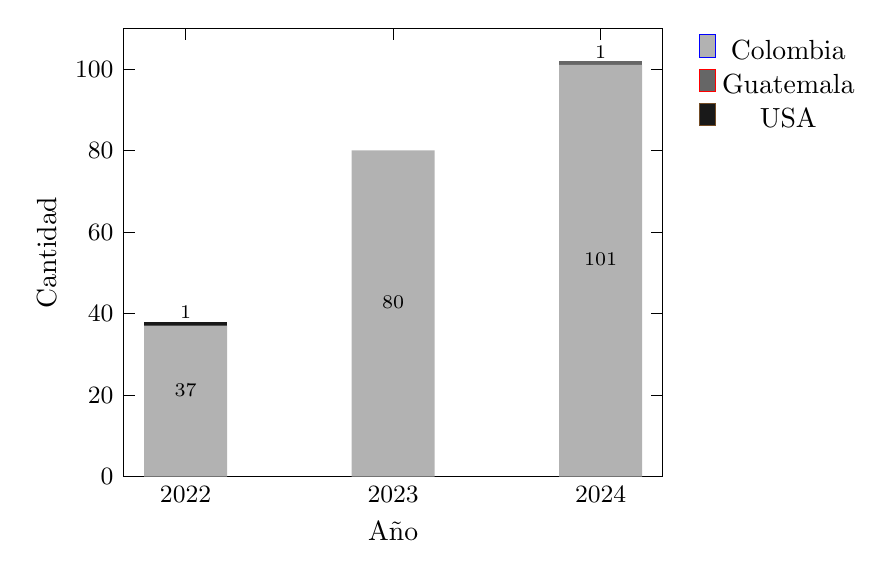
\begin{tikzpicture}
    \begin{axis}[
      ybar stacked,
      bar width=30pt,
      enlarge x limits=0.15,
      ymin=0,
      ymax=110,
      xlabel={Año},
      ylabel={Cantidad},
      symbolic x coords={2022,2023,2024},
      xtick=data,
      legend style={at={(1.05,1)}, anchor=north west, draw=none, fill=none},
      ylabel near ticks,
      xlabel near ticks,
      nodes near coords,
      every node near coord/.append style={
        font=\scriptsize,
        color=black,
        yshift=4pt
      },
      axis line style={black},
      tick style={black},
      tick label style={font=\small}
    ]

      % Escalas de grises para los países
      \addplot+[fill=gray!60, draw=none] coordinates {
        (2022,37) (2023,80) (2024,101)
      };
      \addlegendentry{Colombia}

      \addplot+[fill=black!60, draw=none] coordinates {
        (2022,0) (2023,0) (2024,1)
      };
      \addlegendentry{Guatemala}

      \addplot+[fill=black!90 , draw=none] coordinates {
        (2022,1) (2023,0) (2024,0)
      };
      \addlegendentry{USA}

    \end{axis}
  \end{tikzpicture}
}
{Elaboración propia basada en información interna (2025).}
